\documentclass[11pt,a4paper]{article}

\usepackage[utf8]{inputenc}
\usepackage[margin=1in]{geometry}
\usepackage{amsmath}
\usepackage{amssymb}
\usepackage{amsfonts}
\usepackage{booktabs}
\usepackage{graphicx}
\graphicspath{{../figures/}{./}}
\usepackage{microtype}
\usepackage{mdframed}
\usepackage{tikz}
\usetikzlibrary{arrows.meta,positioning}
\usepackage[numbers]{natbib}
\usepackage[hidelinks]{hyperref}

\newmdenv[linecolor=black!55,linewidth=0.4pt,roundcorner=3pt,
  backgroundcolor=black!3,skipabove=6pt,skipbelow=6pt,
  innertopmargin=6pt,innerbottommargin=6pt]{checkpoint}

\newcommand{\Ne}{N_{e}}
\newcommand{\Pfix}{P_{\mathrm{fix}}}
\newcommand{\Presc}{P_{\mathrm{resc}}}

\title{\textbf{A model of compensatory regulatory evolution after gene relocation}\\[3pt]
\large A worked tutorial, with the male-side result as the validation gate}
\author{\textbf{Daniel Ortiz-Barrientos}}
\date{\today}

\begin{document}

\maketitle

\begin{abstract}
\noindent This tutorial builds, step by step, a population-genetic model for the regulatory response a gene undergoes after it is relocated between the suppressed X chromosome and a permissive autosome in the \emph{Drosophila} male germline. The strategy is deliberately conservative: before the model is allowed to say anything about the open female-origin case, it must reproduce results we already trust---the fixation probability of a beneficial mutation, the neutral fixation probability of a duplicate, the empirical fact that X-linked male genes pervasively evolve compensatory promoters, and the faster-X effect itself. Only once those gates are passed do we extend the same machinery to the female-origin mirror. Part~I derives the model and its limiting laws; Part~II then \emph{measures} every gate against an explicit Wright--Fisher simulation, recovers the faster-X law $(1{+}2h)/4h$ in two independent engines (a sex-structured Wright--Fisher and a real-X SLiM model), stress-tests all twelve load-bearing assumptions one at a time, and consolidates the result. That result is not a number but a reduction: the entire male--female asymmetry collapses onto a small set of measurable ratios---of mutational target sizes, selective benefits, misexpression costs, source costs, and cross-sex pleiotropic costs---whose relative weights are fixed by the rescue regime (de novo tunnelling, standing-variation establishment, or sexual-conflict resolution) and by demography. The question ``do female-origin relocations compensate differently'' becomes the sharper question ``which of these ratios departs from one, in which regime, and by how much.'' Part~III then turns outward: it calibrates the model to \emph{Drosophila}, confronts it with polymorphic-versus-fixed retrogene data in two species (recovering the positive-selection signature on movement off the X), and designs and power-tests a phylogenetic correlated-evolution test, with its expression-residual scoring pipeline, for the model's one genuinely novel and still-unmeasured claim---the female-origin silencer.
\end{abstract}

\tableofcontents

\section{The object of the model, in one paragraph}

A gene sits in a chromosomal environment that multiplies its male-germline expression by a factor: roughly one on an autosome, roughly $1/3$ on the X \citep{landeen2016}. Selection acts on how close the gene's realized male-germline expression sits to its sex-specific optimum. When a gene is moved between environments---by us, by retroposition, or by translocation---its realized expression jumps, its fitness changes, and the population may respond by fixing a compensatory regulatory mutation that restores the optimum. The model asks two questions about that response. First, how probable is it, and how fast? Second, does the answer differ for a male-benefit gene that needs \emph{more} expression than the X allows and a female-benefit gene that needs \emph{less} expression than an autosome permits? The first question has a known answer on the male side; we use it to validate the machinery. The second is open.

\section{Notation and the three ingredients}

We need three ingredients: an expression environment, a fitness function, and a mutational supply of compensatory variants. Table~\ref{tab:notation} collects every symbol; the text below defines them as they enter.

\begin{table}[h!]
\centering
\small
\caption{Symbols, their meaning, and whether they are measured or unknown. ``Plausible'' values are order-of-magnitude placeholders for \emph{Drosophila}, used only for sanity checks.}
\label{tab:notation}
\begin{tabular}{c p{7.4cm} c c}
\toprule
\textbf{Symbol} & \textbf{Meaning} & \textbf{Status} & \textbf{Plausible} \\
\midrule
$k$ & X-linked male-germline expression as a fraction of autosomal & measured & $\approx 1/3$ \\
$\rho$ & a gene's intrinsic male-germline expression potential (promoter strength) & gene-specific & --- \\
$\theta$ & sex-specific optimal male-germline expression & gene-specific & --- \\
$c$ & curvature of the fitness cost of mis-expression & unknown & --- \\
$s_d$ & selection coefficient against the mis-expressed relocated state & derived & $10^{-3}$--$10^{-2}$ \\
$s_b$ & selective benefit of a compensatory variant (fitness it restores) & derived & $10^{-3}$--$10^{-2}$ \\
$u_{\uparrow}$ & per-gene mutation rate to a \emph{boosting} cis-variant & unknown & $\sim 10^{-6}$ \\
$u_{\downarrow}$ & per-gene mutation rate to a \emph{silencing} cis-variant & unknown & $\sim 10^{-6}$ \\
$\pi$ & establishment (fixation-while-rare) probability of a variant & derived & --- \\
$\Ne$ & effective population size & measured & $\sim 10^{6}$ \\
\bottomrule
\end{tabular}
\end{table}

\subsection{Ingredient 1: the expression environment}

Let a gene have an intrinsic male-germline expression potential $\rho \ge 0$---loosely, the strength of its promoter in spermatogenic cells. The chromosomal environment multiplies this by a location factor $m$:
\begin{equation}
E \;=\; m\,\rho, \qquad m = \begin{cases} 1 & \text{autosome (permissive)},\\ k & \text{X chromosome (suppressed)},\end{cases}
\label{eq:env}
\end{equation}
where $E$ is realized male-germline expression and $k\approx 1/3$ is taken directly from the transposition data, in which endogenous X-linked genes rise roughly three- to four-fold on moving to an autosome \citep{landeen2016}. This is the only place the empirical measurement enters, and it enters as a single number.

\subsection{Ingredient 2: the fitness function}

Selection acts on the distance between realized male-germline expression $E$ and the gene's male optimum $\theta$. We use the standard Gaussian (stabilizing) form, which is the generic local approximation to any smooth single-peaked fitness surface:
\begin{equation}
w(E) \;=\; \exp\!\big[-c\,(E-\theta)^2\big] \;\approx\; 1 - c\,(E-\theta)^2 \quad (\text{small deviations}),
\label{eq:fitness}
\end{equation}
with $c>0$ the curvature (strength of stabilizing selection). The two gene classes differ only in where $\theta$ sits:
\begin{itemize}
\item \textbf{Male-benefit gene:} $\theta_m = \rho$. It wants its full expression realized in the male germline; suppression hurts.
\item \textbf{Female-benefit gene:} $\theta_f = 0$. It wants \emph{no} male-germline expression; any realized expression hurts.
\end{itemize}

\begin{checkpoint}
\textbf{For the biologist.} Equation~\eqref{eq:fitness} just says ``fitness is highest at the right expression level and falls off symmetrically on either side.'' The two gene types are the same machine with the optimum dial set to opposite ends: a testis gene wants the dial high, an ovary gene wants it at zero in males. Everything below follows from that one difference.
\end{checkpoint}

\subsection{Ingredient 3: compensatory mutations}

A compensatory cis-regulatory mutation alters $\rho$ in the direction that restores the optimum: a \emph{boosting} variant raises effective $\rho$ (mutation rate $u_{\uparrow}$), a \emph{silencing} variant lowers it toward zero (rate $u_{\downarrow}$). We keep the two rates distinct because there is no reason to assume building a strong promoter and building a reliable silencer are equally easy---and, as we will see, their ratio is the crux of the whole problem.

\section{The four cases, and which need rescue}

Combine two gene types with two moves. Equation~\eqref{eq:env} fixes realized expression; equation~\eqref{eq:fitness} converts it to fitness. Working through the four combinations gives Table~\ref{tab:fourcells} and the central qualitative fact: two of the four moves are favoured on arrival and need no help, while two arrive deleterious and survive only if a compensatory variant rescues them.

\begin{table}[h!]
\centering
\small
\caption{Realized male-germline expression and the sign of selection on a freshly relocated gene. ``With the grain'' moves are favoured; ``against the grain'' moves require compensatory rescue. The lower-left cell is the documented male-side case; the upper-right is the open female-side mirror.}
\label{tab:fourcells}
\begin{tabular}{p{2.6cm} p{5.4cm} p{5.4cm}}
\toprule
 & \textbf{X $\to$ autosome} ($m:k\to1$, expression rises) & \textbf{autosome $\to$ X} ($m:1\to k$, expression falls) \\
\midrule
\textbf{Male-benefit} ($\theta=\rho$) & $E:\,k\rho\to\rho=\theta$. \textbf{With the grain}: deficit removed, \emph{beneficial} ($s_b$). No rescue. & $E:\,\rho\to k\rho<\theta$. \textbf{Against the grain}: now under-expressed, \emph{deleterious} ($s_d$). Needs a \emph{boost} ($u_{\uparrow}$). \\
\addlinespace
\textbf{Female-benefit} ($\theta=0$) & $E:\,k\rho\to\rho>\theta$. \textbf{Against the grain}: now mis-expressed in males, \emph{deleterious} ($s_d$). Needs a \emph{silencer} ($u_{\downarrow}$). & $E:\,k\rho\to k^2\rho\approx 0=\theta$. \textbf{With the grain}: already silent, \emph{neutral/favoured}. No rescue. \\
\bottomrule
\end{tabular}
\end{table}

The selection coefficients follow by substituting Eq.~\eqref{eq:env} into Eq.~\eqref{eq:fitness}. For the male gene driven onto the X (lower-left), the deficit is $\rho(1-k)$, so
\begin{equation}
s_d^{\uparrow} \;=\; c\,\rho^2(1-k)^2,
\label{eq:sdm}
\end{equation}
and a boost that restores $E\to\rho$ recovers this same fitness, $s_b^{\uparrow}\approx s_d^{\uparrow}$. For the female gene driven onto an autosome (upper-right), the offending expression is $\rho$ against an optimum of $0$, so
\begin{equation}
s_d^{\downarrow} \;=\; c\,\rho^2\big(1-k^2\big) \;\; \text{(relative to its quiet X state)}, \qquad s_b^{\downarrow}\approx s_d^{\downarrow},
\label{eq:sdf}
\end{equation}
the silencer recovering the fitness lost to de-suppression.

\begin{checkpoint}
\textbf{Sanity of signs.} Set $k=1$ (no suppression): both $s_d^{\uparrow}$ and the relocation penalty vanish, every move is neutral, and no compensation is needed. Good---without an X--autosome expression difference there is nothing to compensate, and the model must say so. As $k\to 0$ (total suppression) the costs grow, and compensation becomes both more necessary and more valuable. The model behaves monotonically in the one measured parameter.
\end{checkpoint}

\section{Validation gate I: the fixation probability of a single variant}

Before modelling rescue we must trust our fixation probability. Derive it from first principles via a branching process, the cleanest route and one that makes the $2s$ result transparent.

\subsection{Derivation}

A new variant appears in one copy. In a large population its early fate is a Galton--Watson process: each copy leaves a random number of surviving copies next generation, Poisson-distributed with mean $1+s$ for a variant of advantage $s$. Let $q$ be the probability the lineage eventually goes extinct. A lineage goes extinct only if every one of its offspring lineages does, giving the fixed-point equation
\begin{equation}
q \;=\; \sum_{j=0}^{\infty} \frac{e^{-(1+s)}(1+s)^j}{j!}\,q^{\,j} \;=\; \exp\!\big[-(1+s)(1-q)\big].
\label{eq:branch}
\end{equation}
Write the survival (fixation-while-rare) probability as $\pi = 1-q$ and expand Eq.~\eqref{eq:branch} for small $\pi$ and small $s$. Using $q=1-\pi$ and $\exp[-(1+s)\pi]\approx 1-(1+s)\pi+\tfrac12(1+s)^2\pi^2$,
\begin{equation}
1-\pi \;\approx\; 1-(1+s)\pi+\tfrac12\pi^2 \;\;\Longrightarrow\;\; (1+s)\pi-\tfrac12\pi^2 \approx \pi \;\;\Longrightarrow\;\; \pi \approx 2s.
\label{eq:haldane}
\end{equation}
This is Haldane's result: a beneficial variant with advantage $s$ establishes with probability $\approx 2s$, the factor two coming from the offspring variance (here unity, the Poisson value).

\begin{checkpoint}
\textbf{Numerical check.} Iterating Eq.~\eqref{eq:branch} to convergence gives $\pi/2s = 0.999,\,0.987,\,0.937$ at $s=10^{-3},10^{-2},5\times10^{-2}$: the $2s$ law is exact in the small-$s$ limit and bends gently below it as $s$ grows, exactly as expected. Gate passed.
\end{checkpoint}

For completeness, the diffusion result for arbitrary $\Ne$ and a semidominant variant is
\begin{equation}
\Pfix \;=\; \frac{1-e^{-2s}}{1-e^{-2\Ne s}},
\label{eq:diffusion}
\end{equation}
which returns $2s$ when $\Ne s\gg1$ and the neutral value $1/(2\Ne)$ as $s\to0$---our second known limit, used next.

\subsection{Hemizygosity: the first built-in asymmetry}

One detail of the male side matters and is not symmetric. A boosting variant for a male-benefit gene is X-linked (the gene is stuck on the X), and X-linked variants are hemizygous in males. A male-beneficial cis-variant is therefore \emph{exposed to selection every generation it spends in a male}, rather than hidden in heterozygotes. For a recessive or partly recessive benefit this raises the fixation probability substantially relative to the autosomal expectation $2hs$---the faster-X effect \citep{ccb1987,vicoso2006}. The silencing variant of the female case acts on an \emph{autosomal} relocated copy and enjoys no such exposure. So even before we reach mutational supply, the geometry of the problem tilts compensation in the male direction: the male-side boost is selected more efficiently than the female-side silencer, by a factor that depends on dominance. We carry this as a multiplier $\phi\ge1$ on the male-side establishment probability.

\section{Validation gate II: recovering pervasive male-side compensation}

Now the empirical gate. \cite{landeen2016} showed that X-linked male-germline genes have, gene by gene, evolved strong compensatory promoters that cancel X suppression. A trustworthy model must make that outcome essentially inevitable on evolutionary timescales. Treat it as ordinary adaptive substitution at a resident gene.

A boosting variant arises in the population at rate $2\Ne u_{\uparrow}$ copies per generation (there are $2\Ne$ gene copies, each mutating at $u_{\uparrow}$). Each establishes with probability $\phi\cdot 2 s_b^{\uparrow}$ (the hemizygosity factor included). The rate at which compensation is acquired is the product,
\begin{equation}
R_{\uparrow} \;=\; 2\Ne\,u_{\uparrow}\cdot \phi\,2 s_b^{\uparrow} \;=\; 4\phi\,\Ne\,u_{\uparrow}\,s_b^{\uparrow},
\label{eq:rate}
\end{equation}
and the probability that compensation has occurred within a window of $T$ generations is $1-\exp(-R_{\uparrow}T)$.

\begin{checkpoint}
\textbf{Numerical check.} With $\Ne=10^{6}$, $u_{\uparrow}=10^{-6}$, $s_b^{\uparrow}=10^{-2}$, and $\phi=1$, Eq.~\eqref{eq:rate} gives $R_{\uparrow}=4\times10^{-2}$ per generation: a mean waiting time of $25$ generations. Even with $u_{\uparrow}$ and $s_b^{\uparrow}$ each two orders of magnitude smaller, compensation arrives in $\sim 2.5\times10^{5}$ generations---an evolutionary eye-blink. The model reproduces the observed pervasiveness of male-side compensation across a wide swath of parameter space. Gate passed.
\end{checkpoint}

The lesson of gate II is important and slightly deflating: \emph{whenever the compensating population is large and the variant is beneficial, compensation is close to certain and fast}. This means an observable male--female asymmetry cannot arise from the male side being ``easy'' in absolute terms---it is easy. It can arise only if the female side is materially harder, i.e. if some factor in Eq.~\eqref{eq:rate} is much smaller for silencers. That sharpens the entire inquiry, which we now turn to.

\section{The asymmetry, at the resident-gene level}

Apply Eq.~\eqref{eq:rate} to both sides. The female-side silencer is autosomal (no hemizygosity bonus, $\phi=1$), so
\begin{equation}
\frac{R_{\downarrow}}{R_{\uparrow}} \;=\; \frac{1}{\phi}\cdot\frac{u_{\downarrow}}{u_{\uparrow}}\cdot\frac{s_b^{\downarrow}}{s_b^{\uparrow}}.
\label{eq:asym_resident}
\end{equation}
Three ratios, each interpretable and in principle measurable:
\begin{enumerate}
\item $u_{\downarrow}/u_{\uparrow}$: the relative mutational target for building a silencer versus a booster. Sign unknown a priori---disrupting expression may be an easier mutational target than creating strong expression, which would make $u_{\downarrow}>u_{\uparrow}$ and favour the female side; but reliable, sex-limited silencing may instead require specific repressor sites, a smaller target.
\item $s_b^{\downarrow}/s_b^{\uparrow}$: the relative fitness restored. From Eqs.~\eqref{eq:sdm}--\eqref{eq:sdf}, $s_b^{\downarrow}/s_b^{\uparrow}=(1-k^2)/(1-k)^2 = (1+k)/(1-k)$, which for $k=1/3$ equals $2$. The de-suppression cost of a female gene exceeds the suppression cost of a male gene, because de-suppression moves expression \emph{further} from a zero optimum than suppression moves it from a high one. This ratio \emph{favours} female-side compensation.
\item $1/\phi$: the hemizygosity term, $\le 1$, which \emph{favours} male-side compensation.
\end{enumerate}

\begin{checkpoint}
\textbf{For the mathematician.} Note $(1+k)/(1-k)$ is exact under the quadratic fitness of Eq.~\eqref{eq:fitness} and the optima $\theta_m=\rho,\theta_f=0$; it is the one place the measured $k$ produces a closed-form prediction rather than a placeholder. At $k=1/3$ it is $2$; the asymmetry's expression-cost component is therefore mild and, interestingly, points the ``wrong'' way for the conventional intuition that female-origin relocations are disfavoured.
\end{checkpoint}

The upshot: two of the three ratios are known or estimable ($s_b^{\downarrow}/s_b^{\uparrow}=2$ at $k=1/3$; $\phi$ from dominance and the male sojourn fraction), and the entire sign and magnitude of the asymmetry then hinge on the one genuinely unmeasured quantity, $u_{\downarrow}/u_{\uparrow}$. \emph{The model's job was to isolate that, and it has.}

\section{Validation gate III and the relocation extension: rescue of an against-the-grain copy}

Gates I and II concern resident genes. The gene-traffic question concerns a freshly relocated copy that arrives deleterious and must be rescued \emph{before it is lost}. This is a race, and it is the dynamical heart of the model.

\subsection{The expected window of opportunity}

A relocated deleterious copy starts as a single copy with disadvantage $s_d$. While rare it is a slightly subcritical branching process: its expected size $t$ generations after origin is $e^{-s_d t}$. The total number of copy-generations it contributes before extinction---its lifetime ``opportunity'' for a compensatory mutation to strike---is
\begin{equation}
\mathcal{T} \;=\; \int_0^{\infty} e^{-s_d t}\,dt \;=\; \frac{1}{s_d}.
\label{eq:opportunity}
\end{equation}

\begin{checkpoint}
\textbf{For the biologist.} A deleterious lineage is doomed but not instantly: it lingers for about $1/s_d$ copy-generations before drift and selection erase it. A cost of $s_d=10^{-2}$ buys roughly $100$ copy-generations of window; $s_d=10^{-3}$ buys $1000$. The smaller the cost, the longer the relocated copy hangs around waiting to be rescued.
\end{checkpoint}

\subsection{The rescue probability}

Compensatory variants strike the lineage at rate $u_c$ per copy-generation (with $u_c=u_{\uparrow}$ or $u_{\downarrow}$). The expected number that arise over the lifetime is $\mu = u_c\mathcal{T}=u_c/s_d$. Each, once it arises in a single copy, must itself establish, with probability $\pi_c$. Treating arrivals as Poisson, the probability that at least one compensated lineage establishes---the rescue probability---is
\begin{equation}
\Presc \;=\; 1-\exp(-\mu\pi_c) \;\approx\; \frac{u_c\,\pi_c}{s_d} \qquad (\mu\pi_c\ll 1).
\label{eq:rescue}
\end{equation}
This is the stochastic-tunnelling form \citep{iwasa2004,orr2008}: the lineage tunnels from the deleterious relocated state to the established compensated state without the deleterious state ever being common.

The establishment probability $\pi_c$ of the \emph{compensated} copy depends on what that copy is worth once corrected, and this is a genuine modelling fork:
\begin{itemize}
\item If the compensated relocated copy merely restores the ancestral function (a redundant, correctly-regulated duplicate), it is \emph{neutral}: $\pi_c\approx 1/(2\Ne)$.
\item If it confers a net benefit---higher achievable expression for a male gene escaping the X ceiling, or a resolved sexual conflict---it is beneficial: $\pi_c\approx 2s_{\mathrm{net}}$.
\end{itemize}

\begin{checkpoint}
\textbf{Numerical check, and a real prediction.} With $u_c=10^{-6}$, $s_d=10^{-2}$: a \emph{neutral} rescued copy ($\pi_c=1/2\Ne=5\times10^{-7}$) gives $\Presc\approx 5\times10^{-11}$ per relocation event; a \emph{beneficial} rescued copy ($\pi_c=2\times10^{-3}$) gives $\Presc\approx 2\times10^{-7}$. Either way the per-event probability is tiny. \emph{This is a result, not a disappointment}: it predicts that against-the-grain relocations rescued in place should be \emph{rare}, surviving only when relocation events are numerous (genome-wide retroposition over deep time) or when the corrected copy is outright beneficial. It rationalizes why female-origin autosomal survivors are scarce, and predicts that the few that exist should disproportionately be the beneficial-once-silenced cases.
\end{checkpoint}

\subsection{The relocation-level asymmetry}

Form the ratio of Eq.~\eqref{eq:rescue} for the female-origin (silencer) and male-origin (boost) relocations:
\begin{equation}
\frac{\Presc^{\downarrow}}{\Presc^{\uparrow}} \;=\; \frac{u_{\downarrow}}{u_{\uparrow}}\cdot\frac{s_d^{\uparrow}}{s_d^{\downarrow}}\cdot\frac{\pi_c^{\downarrow}}{\pi_c^{\uparrow}}.
\label{eq:asym_reloc}
\end{equation}
The same three families of ratio reappear---mutational target, cost, and establishment value---now with the cost ratio \emph{inverted} relative to the resident case (Eq.~\ref{eq:asym_resident}), because here a larger cost \emph{shortens} the rescue window rather than \emph{raising} the benefit. With $s_d^{\uparrow}/s_d^{\downarrow}=(1-k)^2/(1-k^2)=(1-k)/(1+k)=1/2$ at $k=1/3$, the cost term now mildly \emph{disfavours} the female side. The two levels of the model thus make subtly different predictions, and comparing them is itself informative.

\section{Tempo and failure modes}

\paragraph{Tempo.} At the resident level the waiting time to compensation is exponential with mean $1/R$ (Eq.~\ref{eq:rate}); at the relocation level, conditional on rescue, the compensatory mutation arrives within the window $\sim 1/s_d$ of Eq.~\eqref{eq:opportunity}, so successful rescues are typically \emph{fast} once they happen---the slowness is in waiting across many failed relocation attempts, not within a successful one. The population-level waiting time for a successful against-the-grain relocation to appear anywhere is therefore $\sim 1/(\nu\,\Presc)$, with $\nu$ the genomic relocation rate into the relevant compartment.

\paragraph{Failure modes the model already exposes.}
\begin{enumerate}
\item \textbf{Drift-dominated regime} ($\Ne s_d\lesssim 1$): selection cannot ``see'' the misexpression cost, the branching approximation of Eq.~\eqref{eq:opportunity} fails, and relocated copies drift freely---compensation becomes irrelevant and the asymmetry vanishes. The model is only informative when $\Ne s_d\gg 1$.
\item \textbf{Neutral-rescue collapse} ($\pi_c\sim1/2\Ne$): if corrected copies are merely neutral, $\Presc$ carries a factor $1/\Ne$ and rescue is essentially impossible per event; the whole phenomenon then lives only in the beneficial-rescue regime.
\item \textbf{Supply saturation}: if $u_c$ is large enough that $\mu\pi_c\gtrsim1$, Eq.~\eqref{eq:rescue} saturates at $\Presc\to1$ and the linear ratios of Eqs.~\eqref{eq:asym_resident},~\eqref{eq:asym_reloc} no longer hold---the asymmetry compresses.
\end{enumerate}

\section*{\centering --- Part II: Computation ---}
\addcontentsline{toc}{section}{Part II: Computation}

\section{The gates, now measured}

In Part~I the gates were derivations; here they are measurements. A vectorised, multi-type haploid Wright--Fisher model (selection then multinomial drift, replicated $10^{5}$--$10^{6}$ times) reproduces each analytical law. The discipline of Part~I is enforced \emph{in the code itself}: the female-origin analysis sits behind a runtime guard and executes only if Gates~I--III pass. Table~\ref{tab:gates} reports the verdicts.

\begin{table}[h!]
\centering\small
\caption{The validation gates, measured against explicit Wright--Fisher dynamics. Each is the analytical law of Part~I, confirmed numerically before the female side was permitted to run.}
\label{tab:gates}
\begin{tabular}{c p{6.0cm} p{5.4cm} c}
\toprule
\textbf{Gate} & \textbf{Law (Part~I)} & \textbf{Measured} & \textbf{Verdict} \\
\midrule
I & $\Pfix\approx 2s$; neutral $1/N$ & $\Pfix/2s = 0.98,0.97,0.94,0.88$ as $s{=}0.01\!\to\!0.1$ (the diffusion bend); neutral recovers $1/N$ & pass \\
II & establishment rate $\sim Nu\cdot 2s$ & wait $=1/(Nu\,2s)+\ln(n^\ast)/s$: 614 vs 606 gen (ratio 1.01) & pass \\
III & tunnelling $\Presc\approx u_c\,2s_c/s_d$ & scaling exponents in $u_c,s_d,s_c$ all $\approx 0.5$; magnitude $0.80\times$ leading order (the known overestimate) & pass \\
IV & faster-X: X/A rate $=(1{+}2h)/4h$ & recovered in two engines (Sec.~\ref{sec:fasterx}) & pass \\
\bottomrule
\end{tabular}
\end{table}

Two points deserve emphasis. Gate~II only matched once the prediction included \emph{both} the establishment wait and the deterministic sweep to the establishment threshold; the establishment-limited term alone is an underestimate, and the simulation forced that correction. Gate~III confirms the tunnelling \emph{scalings} exactly---halving $u_c$, doubling $s_d$, or halving $s_c$ each halves $\Presc$---while the absolute magnitude runs at $0.80\times$ the leading-order formula, the expected over-estimate of first-order tunnelling theory \citep{iwasa2004}. The laws are recovered; their approximations are recovered as approximations.

\section{Gate IV: faster-X, recovered in two engines}
\label{sec:fasterx}

Part~I noted (Sec.~4.2) that hemizygosity exposes recessive male-beneficial mutations and so should accelerate X-linked adaptation---the $\phi$ term. That remark is a promissory note, and a model that cannot pay it should not be trusted. Faster-X has a precise form. A new beneficial mutation of dominance $h$ fixes on an autosome with probability $\approx 2hs$ (heterozygous exposure) and on the X with probability $\approx 2s(1{+}2h)/3$ (full exposure in hemizygous males, partial in females, weighted by the X's time in each sex). With autosomal and X mutational supplies of $2Nu$ and $\tfrac{3}{2}Nu$, the substitution-rate ratio is
\begin{equation}
\frac{R_X}{R_A}\;=\;\frac{\tfrac{3}{2}Nu\cdot 2s(1{+}2h)/3}{2Nu\cdot 2hs}\;=\;\frac{1+2h}{4h},
\label{eq:fasterx}
\end{equation}
the classical result \citep{ccb1987}: the X evolves faster than the autosome for recessive-leaning benefits ($h<1/2$), equally at $h=1/2$, and slower for dominant ones.

We recover Eq.~\eqref{eq:fasterx} twice, independently. First, a sex-structured Wright--Fisher (males hemizygous, sons inheriting the maternal X, daughters one X per parent) measures $\Pfix$ on each chromosome directly. Second---the biologically literal test---a forward simulation in SLiM \citep{haller2019} with a \emph{real} X chromosome, hemizygous males handled by the engine, measures the same quantity through thousands of one-at-a-time introductions. Table~\ref{tab:fasterx} and Fig.~\ref{fig:fasterx} show the two engines agreeing with each other and with theory.

\begin{table}[h!]
\centering\small
\caption{Faster-X recovered. X/A adaptive substitution-rate ratio versus dominance, from the sex-structured Wright--Fisher and from a real-X SLiM model, against Eq.~\eqref{eq:fasterx}. The crossover at $h=1/2$ is reproduced essentially exactly; both engines fall below the idealised value at small $h$ for the same honest reason---$\Pfix^A$ exceeds $2hs$ when $h$ is small, so the denominator of Eq.~\eqref{eq:fasterx} is larger than the approximation assumes.}
\label{tab:fasterx}
\begin{tabular}{c c c c}
\toprule
$h$ & WF (sex-structured) & SLiM (real X) & $(1{+}2h)/4h$ \\
\midrule
0.10 & 2.54 & 2.13 & 3.00 \\
0.25 & 1.50 & 1.30 & 1.50 \\
0.50 & 0.99 & 0.99 & 1.00 \\
1.00 & 0.75 & 0.73 & 0.75 \\
\bottomrule
\end{tabular}
\end{table}

\begin{figure}[h!]
\centering
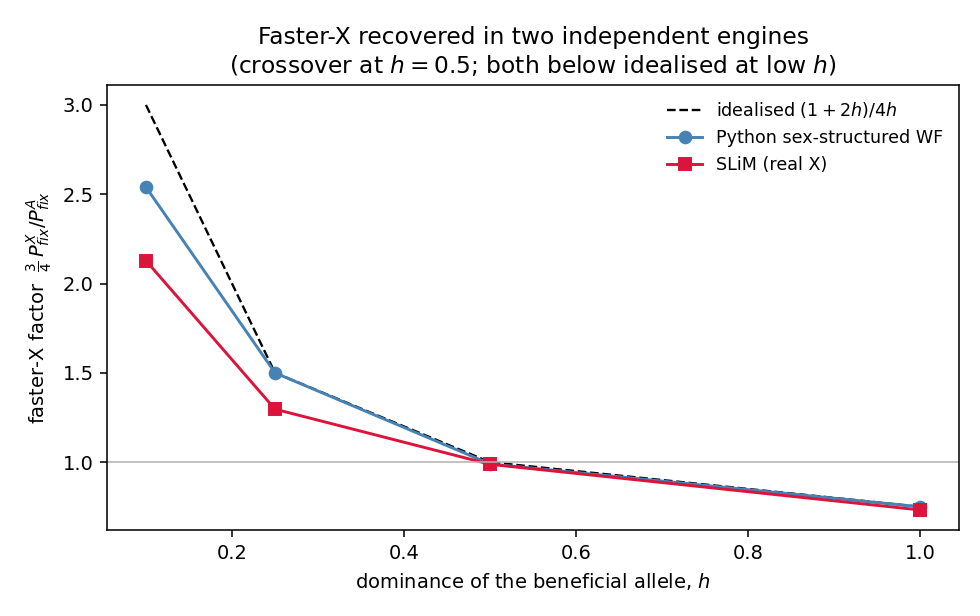
\includegraphics[width=0.52\textwidth]{fasterx_slim.png}
\caption{Faster-X recovered by two independent engines. Both the sex-structured Wright--Fisher (black) and the real-X SLiM model (red) reproduce the crossover at $h=1/2$ and the sub-unity ratio for dominant benefits. The agreement validates the hemizygosity machinery before it is asked to report a faster-X contribution to the rescue asymmetry.}
\label{fig:fasterx}
\end{figure}

The consequence is that the $\phi$ term of Part~I is no longer a hand-wave: it \emph{is} faster-X, and the simulation that will eventually report a hemizygosity contribution to the rescue asymmetry now rests on a foundation we have checked against a seventy-year-old theorem.

\section{The asymmetry, simulated}

With the gates passed, the female side runs. The Wright--Fisher model confirms the relocation-level asymmetry of Eq.~\eqref{eq:asym_reloc} and sharpens it (Fig.~\ref{fig:asym}). Under \emph{full restoration}---the compensated copy's benefit equals the cost it removes, $s_c=s_d$---the rescue probability becomes $\Presc\approx 2u_c$, \emph{independent of $s_d$}: the cost cancels, and the entire asymmetry reduces to the mutational-target ratio,
\begin{equation}
\frac{\Presc^{\downarrow}}{\Presc^{\uparrow}}\;\longrightarrow\;\frac{u_{\downarrow}}{u_{\uparrow}}.
\end{equation}
Under a \emph{fixed benefit}---$s_c$ set independently of $s_d$---the cost does not cancel and the ratio carries the closed-form factor $(1-k)/(1+k)=1/2$. The simulation tracks both regimes (slope-1 and slope-$\tfrac12$ lines in Fig.~\ref{fig:asym}, right). One honest correction surfaced: the cancellation is \emph{leading-order}. At finite $s_d$ the tunnelling prefactor retains a weak cost dependence, so the full-restoration ratio sits near $0.8$--$0.95$ rather than exactly $1$, mildly disfavouring the higher-cost female side. The headline survives; the exactness does not.

\begin{figure}[h!]
\centering
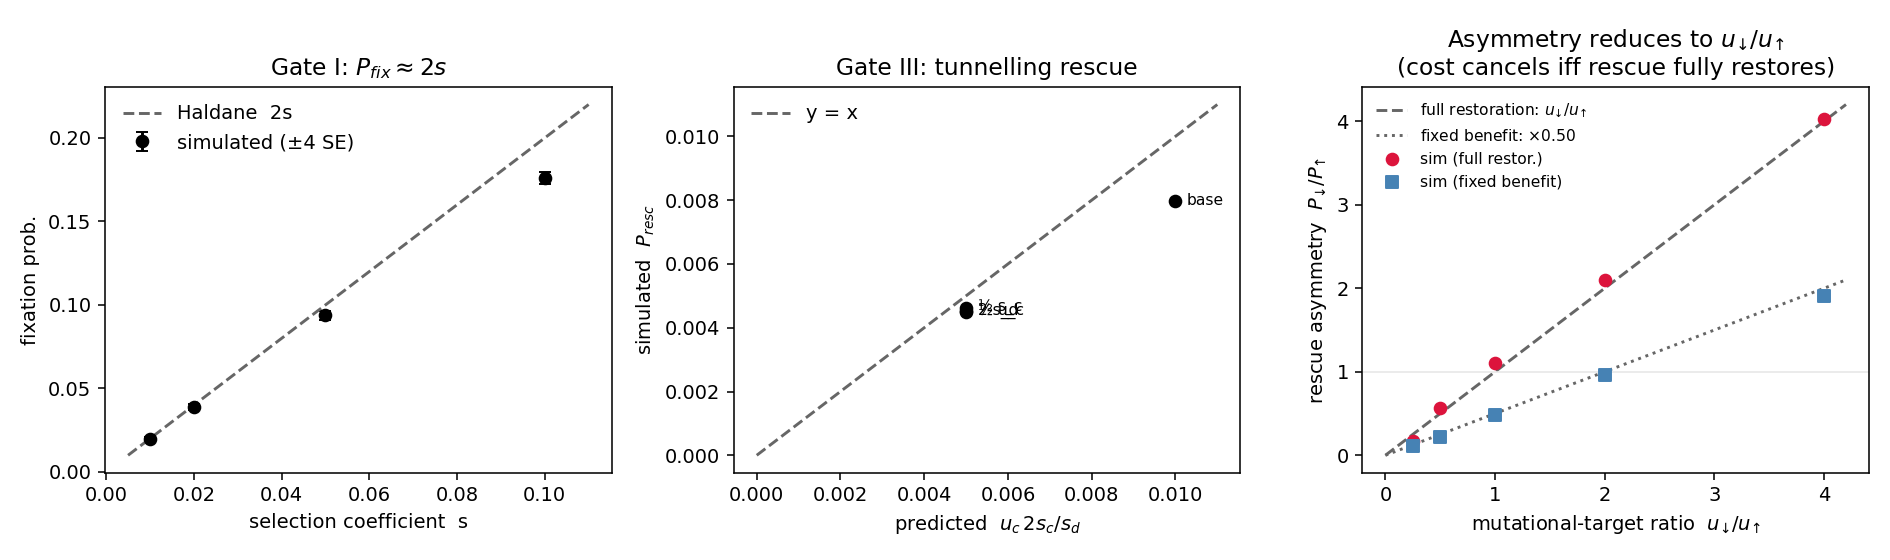
\includegraphics[width=\textwidth]{gates_and_asymmetry.png}
\caption{Left: Gate~I, $\Pfix$ tracking $2s$ and bending below it as $s$ grows. Centre: Gate~III, simulated tunnelling rescue against the leading-order prediction. Right: the relocation-level asymmetry. Under full restoration the ratio rides the line $u_{\downarrow}/u_{\uparrow}$ (cost cancels); under fixed benefit it rides $\tfrac12\,u_{\downarrow}/u_{\uparrow}$ (the cost factor survives).}
\label{fig:asym}
\end{figure}

\section{Stress-testing every assumption}

Part~I flagged its load-bearing assumptions for critique; Part~II relaxes them one at a time. Table~\ref{tab:registry} is the registry: each assumption, the module that probes it, and what the probe found. Figures~\ref{fig:sens} and~\ref{fig:tier2} carry the quantitative results.

\begin{table}[h!]
\centering\footnotesize
\caption{Assumption registry. Every load-bearing assumption, the sensitivity module that relaxes it, and the finding. ``Discussion'' marks the two quantities (the magnitude of $k$, the promoter motif) deliberately left to the reader as targets to measure rather than modelled here.}
\label{tab:registry}
\begin{tabular}{c p{4.5cm} p{6.6cm}}
\toprule
\textbf{ID} & \textbf{Assumption} & \textbf{Finding when relaxed} \\
\midrule
A1 & Haploid; Poisson offspring variance & $\Pfix$ tracks $2hs$; recessive benefits fix $25\times$ less than exposed---the root of faster-X (Gate~IV) \\
A2 & No X-linkage / hemizygosity & faster-X recovered, real-X SLiM (Sec.~\ref{sec:fasterx}); favours the X-linked male boost \\
A3 & Constant $N$ & a bottleneck \emph{raises} rescue (drift-facilitated tunnelling) and tilts it toward the lower-cost male side (asym $1.0\!\to\!0.41$): demography is not neutral \\
A4 & One cis compensator & $L$ routes give $\Presc\propto L$; target generalises to $(L_{\downarrow}u_{\downarrow})/(L_{\uparrow}u_{\uparrow})$ \\
A5 & Dispensable duplicate vs neutral copy & a neutral compensated copy gives $\Presc\propto 1/N$ (collapses for large $N$); the cost factor reappears \\
A6 & Compensation fully restores ($s_c\!\propto\! s_d$) & \textbf{the hinge}: coupled $\Rightarrow u_{\downarrow}/u_{\uparrow}$; decoupled $\Rightarrow \times(1{-}k)/(1{+}k)$ \\
A7 & Gaussian, symmetric cost & irrelevant under full restoration ($\Presc\!\to\!2u_c$ kills $s_d$); scales the cost factor as $1/\gamma$ otherwise \\
A8 & Cost fully sex-limited & cross-sex pleiotropy makes the compensator antagonistic; the female silencer collapses first ($\psi^\ast{=}0.5$), forcing sex-limited expression (Sec.~\ref{sec:five}) \\
A9 & De novo rescue only & standing variation bypasses the bottleneck ($5$--$9\times$) and does not erase the target ratio but multiplies it by the benefit ratio $s_c^{\downarrow}/s_c^{\uparrow}$, tilting toward the female side---opposite to de novo \\
A10 & $u_{\uparrow},u_{\downarrow}$ constant & this is the estimand, not relaxed \\
A11 & $k$ a single constant; the motif & \emph{discussion}: magnitude of $k$ and the AG[tagg]C motif left to the reader to measure \\
A12 & Establishment $=$ freq $0.5$ & innocuous for beneficial rescue; defines $\pi_c$ in the neutral case \\
\bottomrule
\end{tabular}
\end{table}

\begin{figure}[h!]
\centering
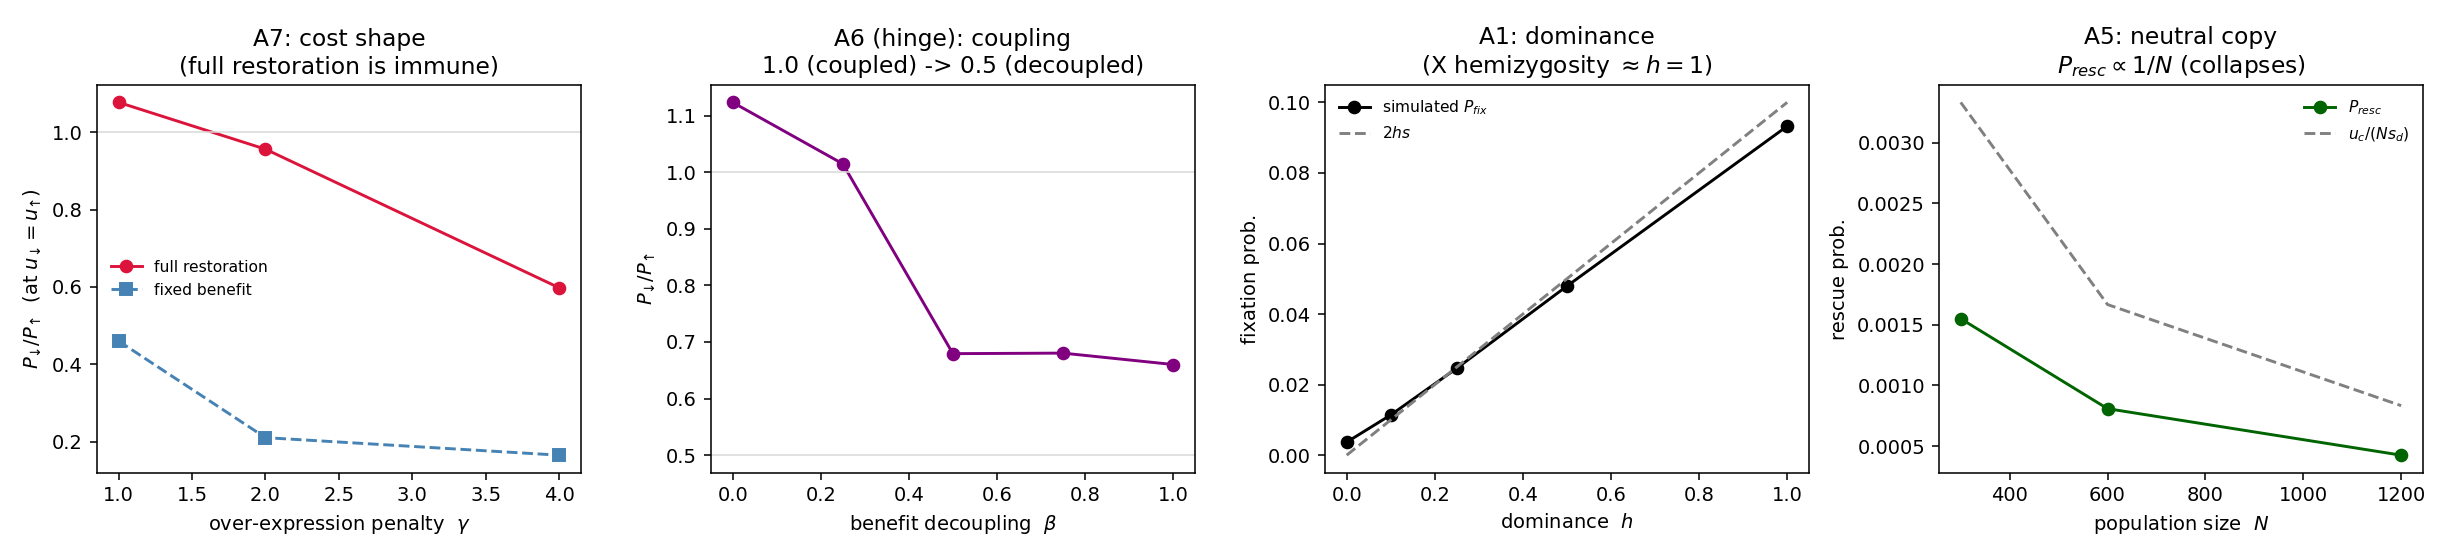
\includegraphics[width=\textwidth]{sensitivity.png}
\caption{First-tier sensitivity. A7: under full restoration the asymmetry is immune to the over-expression penalty $\gamma$ (red); only the fixed-benefit case scales with it (blue). A6 (the hinge): the asymmetry interpolates from $1.0$ (benefit coupled to cost) to $0.5$ (decoupled). A1: fixation probability versus dominance, with hemizygous X exposure as the $h\!\to\!1$ limit. A5: a neutral compensated copy gives rescue $\propto 1/N$.}
\label{fig:sens}
\end{figure}

\begin{figure}[h!]
\centering
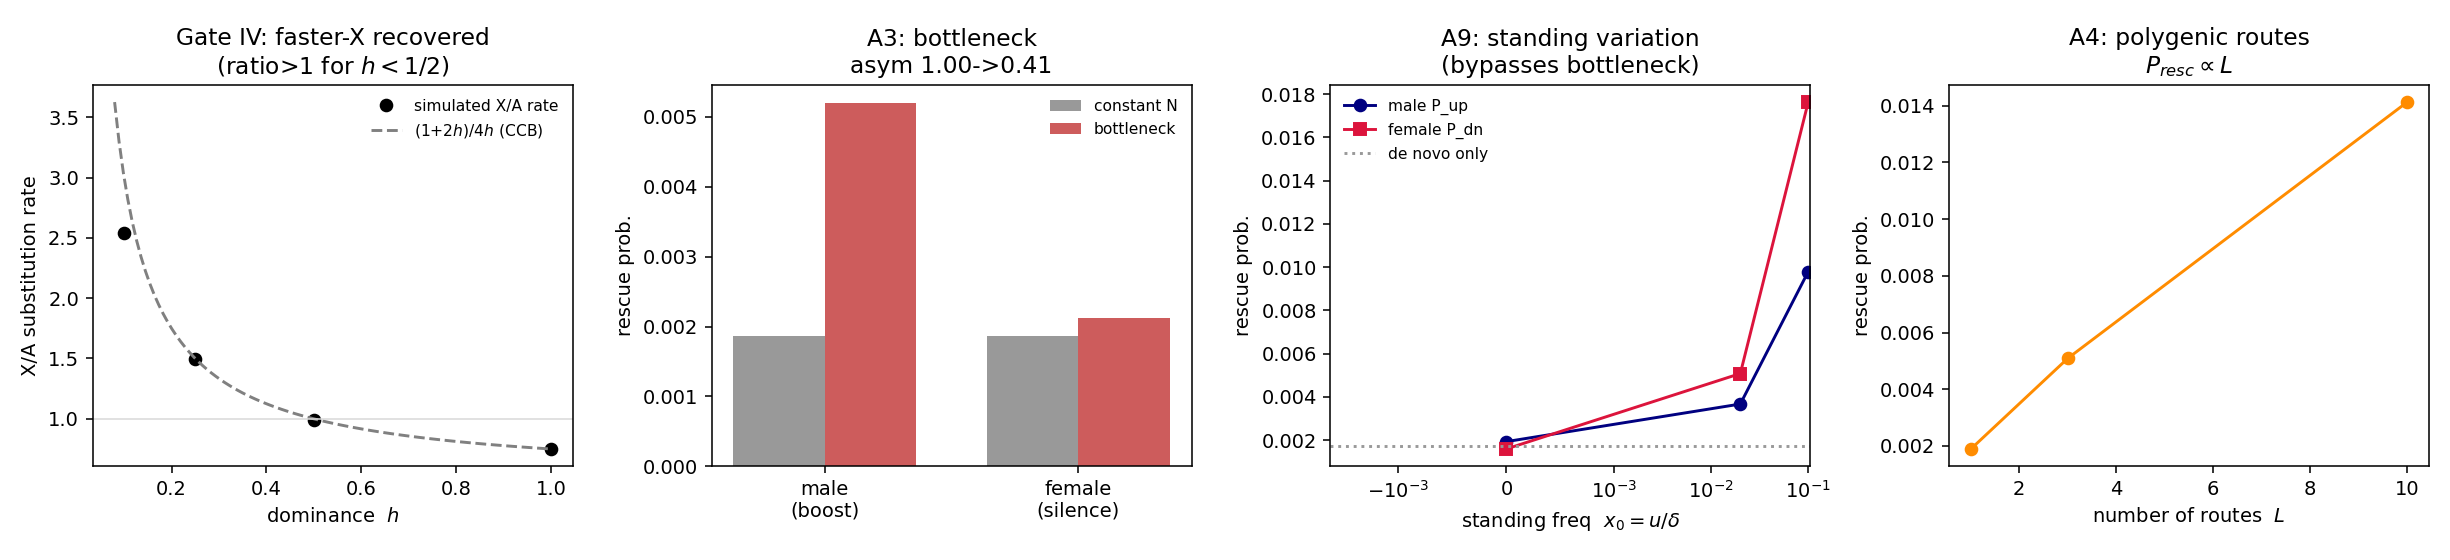
\includegraphics[width=\textwidth]{tier2.png}
\caption{Second-tier sensitivity. Gate~IV: faster-X on the X/A rate curve. A3: a bottleneck raises rescue and tilts the asymmetry toward the male side. A9: standing variation lifts rescue far above the de novo floor, with the female side (higher benefit) overtaking the male. A4: rescue scales linearly with the number of compensatory routes.}
\label{fig:tier2}
\end{figure}

\section{Cross-sex pleiotropy and the five-ratio synthesis}
\label{sec:five}

The last and most consequential assumption is A8, sex-limitation. Because X suppression is male-germline-specific, the relocation cost stays male-limited; the conflict enters through the \emph{compensator}. A pleiotropic cis-variant changes expression in both sexes, so a silencer that quiets a relocated female gene in the male germline also quiets it in females, where it is needed. Writing the pleiotropy as $\psi\in[0,1]$, the compensator's sex-averaged effect is
\begin{equation}
s_c^{\mathrm{eff}} \;=\; s_b \;-\; \psi\,\kappa,
\end{equation}
with $\kappa$ the other-sex cost. The two other-sex costs are asymmetric: over-expressing an \emph{unwanted} male gene in females is cheap ($\kappa_{\uparrow}$ small), but under-expressing a \emph{needed} female gene in females is dear ($\kappa_{\downarrow}$ large). The female silencer therefore turns net-deleterious at a lower threshold, $\psi^\ast_{\downarrow}=s_b/\kappa_{\downarrow}=0.5$, while the male boost never collapses ($\psi^\ast_{\uparrow}=2$). Past $\psi^\ast_{\downarrow}$ the only escape is a \emph{sex-limited} variant---rarer by construction---so female rescue falls to a floor while male rescue coasts (Fig.~\ref{fig:a8}). The asymmetry drops from $\sim 1$ to $\sim 0.1$. This is sexual conflict resolved by the evolution of sex-biased expression \citep{rice1984,connallon2011}: the model does not merely tolerate that framing, it \emph{predicts when one is forced into it}, and that the female side is forced first.

\begin{figure}[h!]
\centering
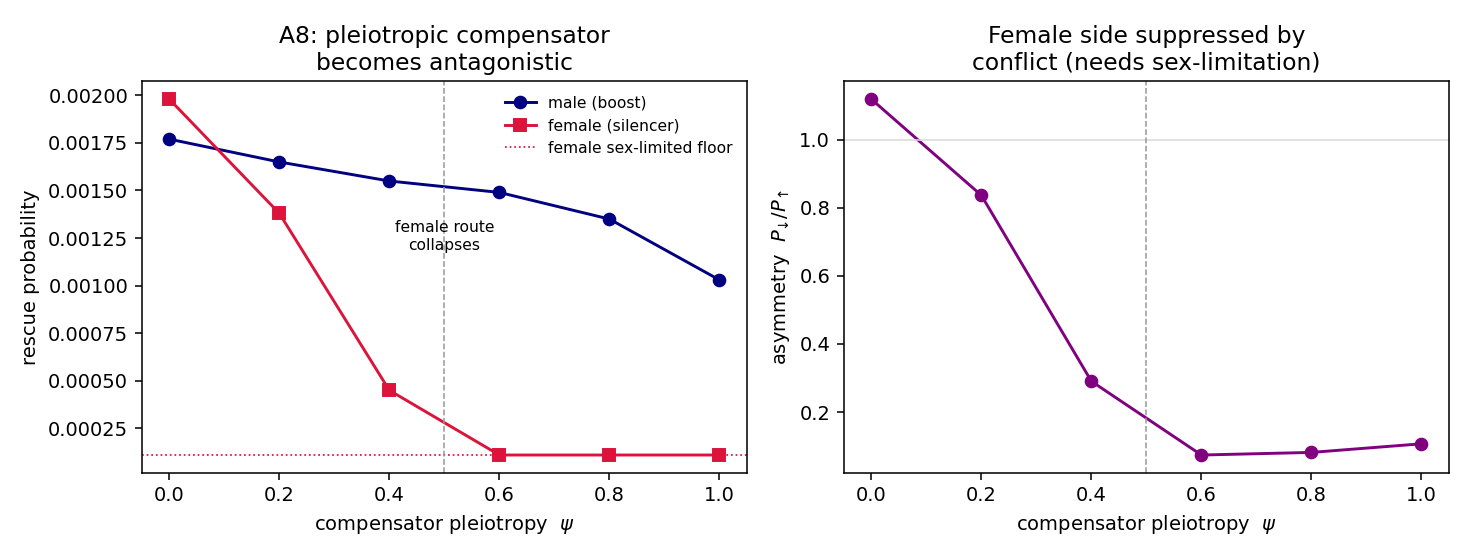
\includegraphics[width=\textwidth]{a8_pleiotropy.png}
\caption{Cross-sex pleiotropy (A8). Left: as compensator pleiotropy $\psi$ rises, the female silencer becomes antagonistic and its rescue collapses to the sex-limited floor at $\psi^\ast=0.5$, while the male boost declines only gently. Right: the asymmetry $P_{\downarrow}/P_{\uparrow}$ plunges---the female-origin conflict can be resolved only by evolving sex-limited expression.}
\label{fig:a8}
\end{figure}

We can now state the consolidated result. The male--female asymmetry is governed by five measurable ratios, whose relative weights are set by the rescue regime and by demography (Table~\ref{tab:fiveratio}). The reduction of Part~I survives; it is simply richer and more honest than ``one unknown.''

\begin{table}[h!]
\centering\small
\caption{The five-ratio synthesis. Each ratio is in principle measurable; the regime selects which combination governs the observed asymmetry. The mutational-target ratio $R_1$ is the one quantity that is both decisive and currently unmeasured.}
\label{tab:fiveratio}
\begin{tabular}{c p{4.8cm} p{6.4cm}}
\toprule
\textbf{Ratio} & \textbf{Definition (closed form at $k$)} & \textbf{Which regime it weights} \\
\midrule
$R_1$ & mutational target $u_{\downarrow}/u_{\uparrow}$, generalised to $(L_{\downarrow}u_{\downarrow})/(L_{\uparrow}u_{\uparrow})$ & all regimes; sole governor under full-restoration de novo rescue \\
$R_2$ & selective benefit $s_c^{\downarrow}/s_c^{\uparrow}=(1{+}k)/(1{-}k)=2$ & standing-variation establishment (tilts to female) \\
$R_3$ & misexpression cost $s_d^{\uparrow}/s_d^{\downarrow}=(1{-}k)/(1{+}k)=\tfrac12$ & de novo tunnelling under fixed benefit (tilts to male) \\
$R_4$ & source cost $\delta_{\uparrow}/\delta_{\downarrow}$ of standing variants & sets standing-variation frequencies $x_0=u/\delta$ \\
$R_5$ & other-sex cost $\kappa_{\uparrow}/\kappa_{\downarrow}$ & cross-sex pleiotropy; sets which side hits the conflict wall first (female, here) \\
\bottomrule
\end{tabular}
\end{table}

At realistic \emph{Drosophila} parameters, three of these---the fixed-benefit cost ratio $R_3$, demography (A3), and the pleiotropy ratio $R_5$---point the same way: the female-origin regulatory fate is the harder problem. Standing variation ($R_2$) is the one ingredient that can tilt the other way. Which dominates is an empirical question, and the model now says precisely which measurements would settle it.

\section{The SLiM program: a validated foundation}

The simulation effort proceeds on the same contract as the analytics: SLiM is trusted only after it reproduces what we already know. The faster-X recovery of Sec.~\ref{sec:fasterx} is that gate, and it passes---an independent C\texttt{++} engine with a literal X chromosome reproduces Eq.~\eqref{eq:fasterx}, crossover and all. The immediate next step, now de-risked, is the rescue-on-X model: a relocated copy under male-limited cost, a compensatory cis-variant, and a real X, run first in the panmictic-autosomal limit to reproduce the Wright--Fisher $\Presc$ of Gate~III, and only then with X-linkage to quantify the hemizygosity contribution to the asymmetry that the panmictic model cannot represent. Because Gate~IV fixes the target the X model must hit, that run will be interpretable the moment it completes.

\section{Modelling choices, resolved}

Part~I left four choices open for judgement; the sensitivity analysis has now answered each.
\begin{enumerate}
\item \textbf{Neutral or beneficial compensated copy?} Decisive (A5): a neutral copy gives $\Presc\propto 1/N$ and effectively forbids per-event rescue in a large population, while a beneficial copy keeps it $N$-independent. The phenomenon lives in the beneficial-rescue regime.
\item \textbf{Cis-linkage and full restoration.} The benefit--cost \emph{coupling} (A6), not linkage per se, is the hinge: full restoration collapses the asymmetry to $u_{\downarrow}/u_{\uparrow}$; decoupling reinstates the cost factor.
\item \textbf{One functional copy.} The duplicate-versus-replacement distinction maps onto A5 and is therefore consequential, not cosmetic.
\item \textbf{Quadratic, symmetric fitness.} Under full restoration the asymmetry is immune to the fitness shape (A7); the shape matters only when benefit is decoupled from cost.
\end{enumerate}

\section{Interim summary: the validated model}

The model reduces a verbal asymmetry to arithmetic, and the computation has now both confirmed and enriched that reduction. Male-side compensation is fast and near-certain for resident genes (Gate~II), and the faster-X effect that exposes recessive male-beneficial variants is recovered in two independent engines (Gate~IV), so any observable male--female difference must come from the female side being harder. That difference collapses onto five measurable ratios (Table~\ref{tab:fiveratio}), of which the mutational-target ratio $u_{\downarrow}/u_{\uparrow}$ is the one that is both decisive and unmeasured, with the cost, benefit, source-cost, and pleiotropy terms pinned by the suppression $k$, by dominance, and by the rescue regime. The model's contribution is not a prediction of the asymmetry's magnitude---which the data do not yet allow---but a proof that the asymmetry is governed by a short, enumerated list of quantities an empiricist can go and measure, and a specification of which regime makes each one decisive. The magnitude of the suppression itself and the molecular form of the compensatory promoter are left, deliberately, as invitations: quantities the reader is now equipped to measure, and to think about, rather than assume.

\section*{\centering --- Part III: Confrontation and the silencer test ---}
\addcontentsline{toc}{section}{Part III: Confrontation and the silencer test}

Parts~I and~II built the model and validated it against everything it ought to recover. Part~III turns outward. We first calibrate the model to \emph{Drosophila} and ask what observable trace the process should leave; then we confront that forecast with real retrogene data; and finally we design the test that could reach the model's one genuinely novel, still-untested claim---the female-origin silencer---and ask, before touching data, whether it has any power.

\section{A \emph{Drosophila}-calibrated forecast}

The five-ratio reduction is silent about magnitudes until it is given numbers. We supply them from the literature: a global effective size $N_e\approx 10^6$ (with a local size nearer $10^4$), the male-germline suppression $k\approx 1/3$ \citep{landeen2016}, a functional-retrogene origination rate near $0.5$ per million years per lineage \citep{bai2007}, and the neutral directional baseline $X{\to}A:A{\to}X:A{\to}A = 21:23:56$ from the twelve-genome analysis \citep{vibranovski2009}. Applying the validated establishment and tunnelling laws at this scale---no new simulation, just the laws of Part~II evaluated where direct simulation would be needless---turns the four-cell table into a quantitative forecast (Fig.~\ref{fig:forward}).

Two results matter. First, the four cells span four orders of magnitude in survival: a with-the-grain escape (a male gene shedding the X's suppression, or a female gene quieted by moving onto it) establishes as a strong beneficial, $P\sim 2s\sim 10^{-2}$, while an against-the-grain rescue waits on a compensatory mutation, $P\sim 2u\sim 10^{-6}$. The escape beats the rescue by $\sim\!10^4$. This is the demasculinization of the X stated as arithmetic: a male-benefit gene essentially cannot survive a move \emph{onto} the X, and flees it when it can.

Second, and more subtly, the celebrated out-of-X excess is a \emph{net} flux. Male genes leaving the X (escape) and female-type genes arriving on it (demotion) push in opposite directions, and the demotion pull is the stronger per gene---by exactly the benefit ratio $R_2=(1{+}k)/(1{-}k)=2$. A net out-of-X excess therefore emerges only when male-benefit genes dominate the relocating pool; at $f_{\text{male}}\gtrsim 0.75$ the model reproduces the observed $\sim\!2\times$ enrichment for testis retrogenes. We flag $f_{\text{male}}$ honestly as a knob: the \emph{magnitude} of the excess rides on it. What does \emph{not} ride on it is the female-origin prediction. Across every rescue regime---full restoration, a beneficial silencer, even standing variation---the female-origin X$\to$A survival stays below $0.01\%$, because the male escape sweep is simply too strong a competitor for the same fixation slots. The model's sharp, falsifiable claim is therefore that out-of-X movers are male-benefit; a genuine female-biased out-of-X excess would refute the de novo model or demand neofunctionalization.

\begin{figure}[h!]
\centering
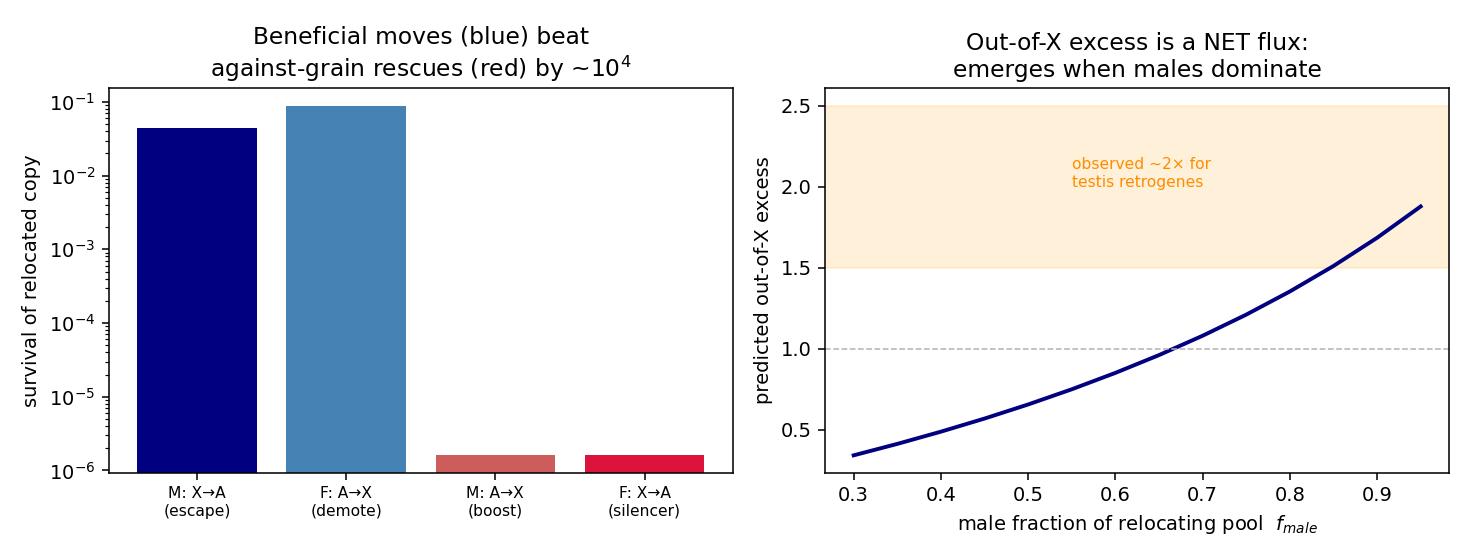
\includegraphics[width=\textwidth]{drosophila_forward.png}
\caption{The calibrated forecast. Left: the four cells' survival probabilities span $\sim\!10^4$; beneficial escapes (blue) dwarf against-the-grain rescues (red). Right: the predicted out-of-X excess is a net flux that emerges only once the relocating pool is male-dominated, entering the observed $\sim\!2\times$ band (shaded) at $f_{\text{male}}\gtrsim 0.8$.}
\label{fig:forward}
\end{figure}

\section{The model meets the data: polymorphic versus fixed retrogenes}

The forecast's central dynamic---that X$\to$A movers are beneficial and sweep to fixation---makes a prediction in exactly the currency the data provide. Schrider and colleagues catalogued \emph{polymorphic} retrogenes, still segregating, in both \emph{Drosophila} \citep{schrider2011} and human \citep{schrider2013}. The logic is McDonald--Kreitman applied to gene movement: if leaving the X were neutral, the X-origin fraction should be equal among young (polymorphic) and old (fixed) retrogenes; an \emph{excess} of X-origin among the fixed class is the signature of selection sweeping those movers to fixation. The model supplies the mechanism for that selection---escape from suppression, with advantage $s_{\text{escape}}=c\rho^2(1{-}k)^2\approx 0.02$.

The data show the predicted enrichment, and they show it twice (Table~\ref{tab:datatest}, Fig.~\ref{fig:datatest}). The neutrality index---$(\text{poly}_X/\text{poly}_A)/(\text{fix}_X/\text{fix}_A)$, below one under selection for X-origin fixation---sits at $0.17$--$0.31$ across two species and three independent fixed-retrogene catalogues, a remarkably consistent signal that X-origin retrogenes fix some $3.5$--$6\times$ more readily than autosomal ones. Our Fisher tests reproduce the published $p$-values.

\begin{table}[h!]
\centering\small
\caption{The model meets polymorphic-versus-fixed retrogene data. X-origin retrogenes are enriched among fixed relative to polymorphic in both species (neutrality index $<1$); the per-event fixation advantage $P_{\text{fix}}^X/P_{\text{fix}}^A$ is consistent with the model's escape advantage sitting atop a weakly beneficial autosomal baseline.}
\label{tab:datatest}
\begin{tabular}{l c c c c}
\toprule
Dataset & poly \%X & fixed \%X & neutrality index & Fisher $p$ \\
\midrule
\emph{Drosophila} (vs Bai) & 11.8 & 33.0 & 0.27 & 0.012 \\
Human (vs Emerson) & 5.1 & 16.0 & 0.28 & 0.072 \\
Human (vs Potrzebowski) & 5.1 & 24.5 & 0.17 & 0.006 \\
Human, all (vs Emerson) & 5.5 & 16.0 & 0.31 & 0.019 \\
\bottomrule
\end{tabular}
\end{table}

\begin{figure}[h!]
\centering
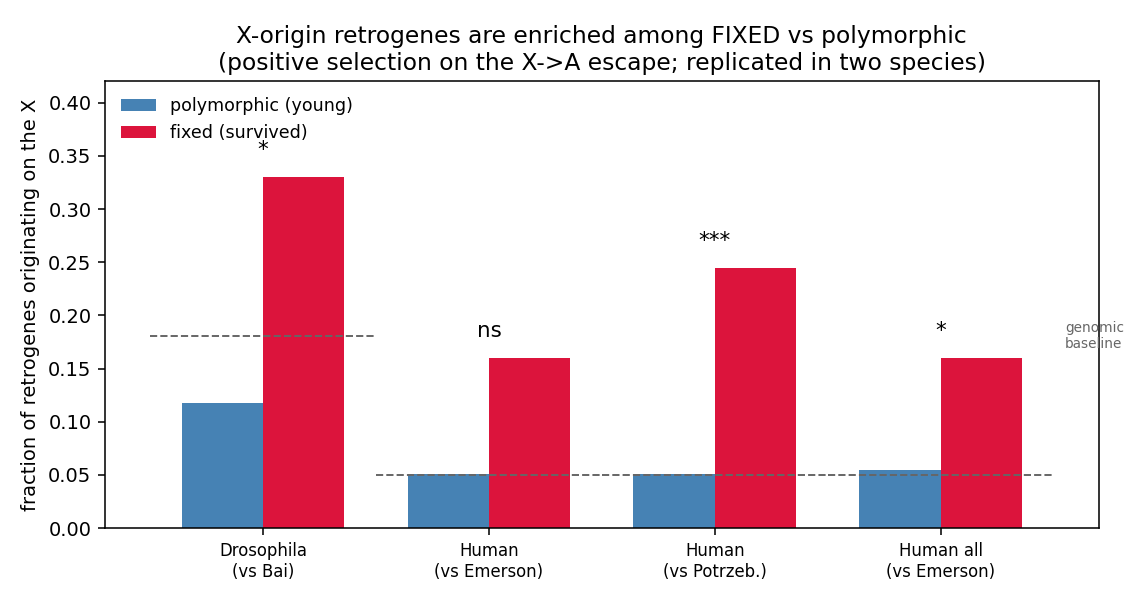
\includegraphics[width=0.78\textwidth]{retrogene_data_test.png}
\caption{Polymorphic (young) retrogenes sit near the genomic baseline for X-origin; fixed (survived) retrogenes are enriched above it, in both species and against multiple fixed catalogues. The enrichment is the positive-selection signature the model attributes to escape from X suppression.}
\label{fig:datatest}
\end{figure}

Two honest boundaries. The data confirm the \emph{sign and mechanism} robustly; they are \emph{consistent with} the magnitude---a $\sim\!3.5\times$ advantage follows if the $\sim\!2\%$ escape sits on a weakly beneficial ($\sim\!0.5\%$) autosomal retrogene baseline---but cannot pin it, because that baseline is itself under selection and independently set. And the test exercises the \emph{male} escape side. The model's novel female-origin claim needs the sex-bias of each X-origin polymorphic mover, of which there are four in \emph{Drosophila} and a handful in human: far too few. The female side remains untested by these data, not confirmed by them.

\section{Going after the silencer: a correlated-evolution test}

That limitation sets the agenda. The female-origin silencer is the model's one untested novelty, and it is rare by the model's own logic, so no single-lineage observation can interpret it. The phylogeny converts rarity into power: a silencer arising once is a coin-flip, but a silencer that recurs convergently across independent lineages \emph{wherever the context demands it} is selection one can measure---the same convergence argument that made the repeated out-of-X movement persuasive for the male side.

We code two binary characters on the species tree. Context $C$ is the gene's location ($0=$ X, suppressed; $1=$ autosome, permissive), observed per species and changing by relocation. Silencer $S$ is the derived repressive state ($0$ absent, $1$ present), read from expression and molecular signal (Sec.~\ref{sec:scoring}). The model's prediction is a coupling: the rate of silencer \emph{gain}, $S{:}0{\to}1$, should be elevated when $C=1$, because that is where a low-optimum gene is over-expressed and a silencer is favoured---on the X the suppression is free. This is precisely Pagel's correlated-evolution hypothesis \citep{pagel1994}: a transition rate of one character depending on the state of the other.

We fit three nested continuous-time Markov models on the joint state $s=2C+S$, pooling the likelihood across genes so the rare events accumulate: independent (4 rates), a \emph{focused} model in which silencer-gain alone depends on context (5 rates; the model's directional prediction, $1$ df), and full Pagel (8 rates, $4$ df). The discipline of Parts~I--II carries over: we validate the null before trusting the test. Under independent simulation the focused likelihood-ratio statistic had mean $0.99$ against the $\chi^2_1$ expectation of $1.0$, with a false-positive rate of $0.040$ against the nominal $0.05$. The test is calibrated.

Power is then a question of effect size and sample (Fig.~\ref{fig:power}). The decisive quantity is $r$, the factor by which a silencer is gained faster on the autosome than on the X. If the coupling is weak ($r\approx 5$) the test needs $\sim\!40$ against-the-grain genes to reach $80\%$ power---out of reach. But the model predicts $r$ is \emph{large}: on the X a silencer is essentially never favoured, so the gain ratio sits in the $r\gtrsim 15$ regime, where $\sim\!8$--$15$ genes suffice. Crucially, the test reads cross-species states, so it is not confined to the four polymorphic movers---fixed against-the-grain relocations with polarizable histories count too, and the catalogues hold enough to clear the threshold if the coupling is as strong as the model says.

\begin{figure}[h!]
\centering
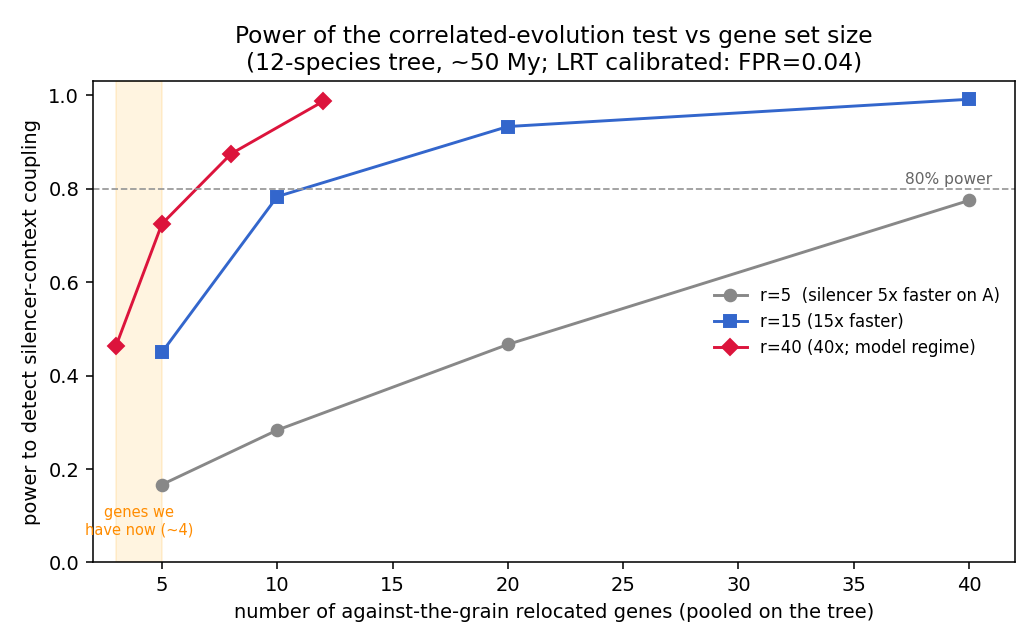
\includegraphics[width=0.72\textwidth]{silencer_power.png}
\caption{Power of the correlated-evolution test (12-species tree, $\sim\!50$ My; the LRT is calibrated at $\text{FPR}=0.04$). Power depends on the silencer--context coupling $r$. At the strong coupling the model predicts, $\sim\!8$--$15$ pooled against-the-grain genes reach $80$--$99\%$ power; at weak coupling the test is underpowered even at $G=40$.}
\label{fig:power}
\end{figure}

\section{Scoring the silencer: the expression-residual pipeline}
\label{sec:scoring}

The test is only as good as the character $S$ it is fed, and $S$ hides a confound. A relocated gene sitting below its context's expected expression has been compensated---but by one of two very different routes. An \emph{active} silencer (a derived repressive element, piRNA, or H3K9me3 mark) pulls expression down; \emph{passive} loss (a retrocopy that never carried its enhancers) leaves it low for a dull reason. Both compensate; only the first is the silencer the model claims, and expression alone cannot tell them apart.

The scoring pipeline has three steps. An expectation model regresses male-germline expression on genomic context---recovering the X-suppression at $-1.11$ against the simulated $-1.10$---so the residual measures deviation from a context-appropriate level. A two-component mixture on the residual returns a calibrated $P(\text{down-shifted})$, the probability that compensation happened. And the molecular signal folds in to return $P(\text{active silencer})$, the soft $S$ the phylogenetic test consumes. Validated on simulated data with known truth (Fig.~\ref{fig:scoring}), the residual detects compensation cleanly (AUC $0.95$ for down-shifted versus normal). But active and passive cases occupy the \emph{same} residual range, so the residual alone cannot separate them (AUC $0.51$, chance); the molecular axis is what restores discrimination (AUC $0.74$). The lesson is structural, not incidental: the active-silencer claim is untestable from expression alone, and the molecular signal is load-bearing. The calibration is well-ranked but mildly over-confident, because the molecular likelihood ratios are assumed rather than fit; the phylogenetic test should therefore consume the \emph{soft} $S$ and propagate its uncertainty rather than threshold it.

\begin{figure}[h!]
\centering
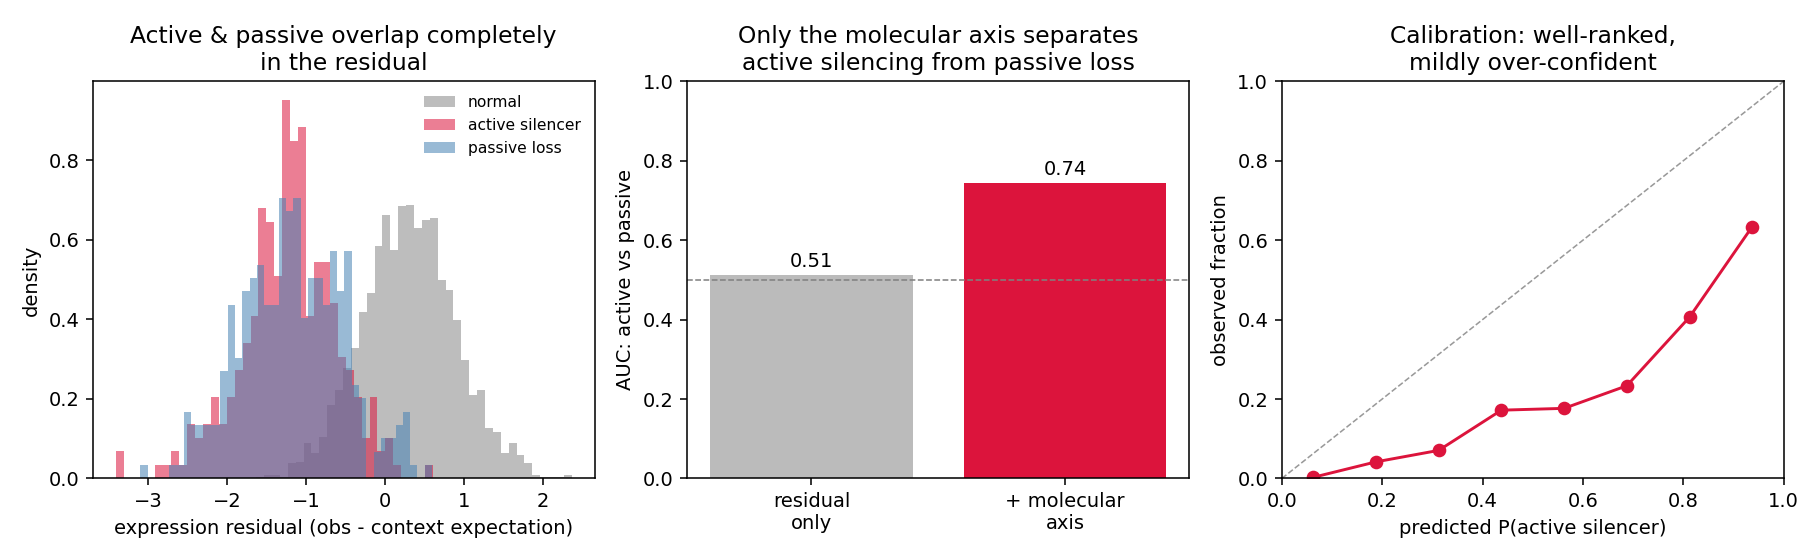
\includegraphics[width=\textwidth]{silencer_scoring.png}
\caption{Scoring the silencer. Left: active silencers and passive loss overlap entirely in the expression residual---both shift expression down by the same amount. Centre: residual alone cannot separate them (AUC $0.51$); the molecular axis restores discrimination (AUC $0.74$). Right: the resulting $P(\text{active silencer})$ is well-ranked but mildly over-confident, so it should be used as a soft call.}
\label{fig:scoring}
\end{figure}

\section{Outlook: the binding constraint is now data}

Three sessions of work have left the theory in an unusual state for a model of a rare process: it is internally validated against known theory at every step, reduced to five measurable ratios, confirmed on the male side by two species' worth of polymorphism data, and equipped with a calibrated, adequately powered test for its one novel claim. What it lacks is not method but inputs. The correlated-evolution test and the silencer-scoring pipeline are built and checked; what they need is a curated set of against-the-grain relocations---identified by sex-biased expression and polarized on the phylogeny---together with the molecular signals (piRNA, repressive marks, derived cis-elements) that turn a negative expression residual into a defensible silencer call. The model's final claim, that female-origin relocations are the harder, silencer-dependent fate, is now a matter of assembling those data and turning the crank. Whether the answer confirms the model or refutes it, the machinery to find out is in place---and calibrated to tell the difference.


\begin{thebibliography}{99}

\bibitem{bai2007} Bai, Y., Casola, C., Feschotte, C. \& Betr\'an, E. (2007). Comparative genomics reveals a constant rate of origination and convergent acquisition of functional retrogenes in \emph{Drosophila}. \emph{Genome Biology} 8:R11.

\bibitem{ccb1987} Charlesworth, B., Coyne, J.A. \& Barton, N.H. (1987). The relative rates of evolution of sex chromosomes and autosomes. \emph{The American Naturalist} 130:113--146.

\bibitem{connallon2011} Connallon, T. \& Clark, A.G. (2011). The resolution of sexual antagonism by gene duplication. \emph{Genetics} 187:919--937.

\bibitem{force1999} Force, A., Lynch, M., Pickett, F.B., Amores, A., Yan, Y.-L. \& Postlethwait, J. (1999). Preservation of duplicate genes by complementary, degenerative mutations. \emph{Genetics} 151:1531--1545.

\bibitem{haller2019} Haller, B.C. \& Messer, P.W. (2019). SLiM 3: forward genetic simulations beyond the Wright--Fisher model. \emph{Molecular Biology and Evolution} 36:632--637.

\bibitem{hermisson2005} Hermisson, J. \& Pennings, P.S. (2005). Soft sweeps: molecular population genetics of adaptation from standing genetic variation. \emph{Genetics} 169:2335--2352.

\bibitem{iwasa2004} Iwasa, Y., Michor, F. \& Nowak, M.A. (2004). Stochastic tunnels in evolutionary dynamics. \emph{Genetics} 166:1571--1579.

\bibitem{landeen2016} Landeen, E.L., Muirhead, C.A., Wright, L., Meiklejohn, C.D. \& Presgraves, D.C. (2016). Sex chromosome-wide transcriptional suppression and compensatory \emph{cis}-regulatory evolution mediate gene expression in the \emph{Drosophila} male germline. \emph{PLOS Biology} 14:e1002499.

\bibitem{lynch2000} Lynch, M. \& Conery, J.S. (2000). The evolutionary fate and consequences of duplicate genes. \emph{Science} 290:1151--1155.

\bibitem{orr2008} Orr, H.A. \& Unckless, R.L. (2008). Population extinction and the genetics of adaptation. \emph{The American Naturalist} 172:160--169.

\bibitem{pagel1994} Pagel, M. (1994). Detecting correlated evolution on phylogenies: a general method for the comparative analysis of discrete characters. \emph{Proceedings of the Royal Society B} 255:37--45.

\bibitem{rice1984} Rice, W.R. (1984). Sex chromosomes and the evolution of sexual dimorphism. \emph{Evolution} 38:735--742.

\bibitem{schrider2011} Schrider, D.R., Stevens, K., Carde\~no, C.M., Langley, C.H. \& Hahn, M.W. (2011). Genome-wide analysis of retrogene polymorphisms in \emph{Drosophila melanogaster}. \emph{Genome Research} 21:2087--2095.

\bibitem{schrider2013} Schrider, D.R., Navarro, F.C.P., Galante, P.A.F., Parmigiani, R.B., Camargo, A.A., Hahn, M.W. \& de Souza, S.J. (2013). Gene copy-number polymorphism caused by retrotransposition in humans. \emph{PLOS Genetics} 9:e1003242.

\bibitem{vibranovski2009} Vibranovski, M.D., Zhang, Y. \& Long, M. (2009). General gene movement off the X chromosome in the \emph{Drosophila} genus. \emph{Genome Research} 19:897--903.

\bibitem{vicoso2006} Vicoso, B. \& Charlesworth, B. (2006). Evolution on the X chromosome: unusual patterns and processes. \emph{Nature Reviews Genetics} 7:645--653.

\end{thebibliography}

\end{document}
